\chapter{Fundamentação Teórica} \label{cap2}


Este capítulo aborda, de forma sucinta, os fundamentos teóricos que foram aplicados no planejamento e implementaçao deste projeto.



\section{Aprendizado de Máquina}

Aprendizado de máquina é uma área da inteligência artificial cujo objetivo é o desenvolvimento de técnicas computacionais sobre o aprendizado, bem como a construção de sistemas capazes de adquirir conhecimento de forma automática. Um sistema baseado em aprendizado trabalha por meio de experiências acumuladas e de soluções bem-sucedidas de problemas anteriores  \cite{monard2003}. Normalmente, algoritmos de aprendizado utilizam experiências anteriores, denominadas amostras de treino, para auxiliar no processo de tomada de decisão.  

De acordo com a característica desses casos ou exemplos têm-se três diferentes modos de aprendizado: supervisionado, não-supervisionado e semi-supervisionado. O que distingue esses modos de aprendizado é a presença ou não do atributo classe, que rotula os exemplos do conjunto de dados fornecido ao algoritmo, denominado conjunto de treinamento. No aprendizado supervisionado, esse rótulo é conhecido, enquanto que no aprendizado não-supervisionado os exemplos não estão previamente rotulados. Já no aprendizado semi-supervisionado, o conjunto de treinamento consiste de uns poucos exemplos rotulados e muitos não rotulados\cite{chappelle2006}. O escopo deste trabalho se encontra no aprendizado supervisionado. 


\subsection{Aprendizado Supervisionado}
O objetivo do aprendizado supervisionado é construir um modelo que consegue fazer predição através de instancias de uma base de dados rotuladas. Cada instância da base de dados é representado por um conjunto de características. Na Tabela \ref{table-dataset} é mostrada a estrutura de uma base de dados.
A base de dados é representada por um conjunto $E={E_1,E_2,...,E_N}$  cada instância está relacionada com um rótulo $y_N$. As colunas $A_1$ até $A_N$ se referem as características de cada instância.

A idéia da aprendizagem supervisionada é o conseguir encontrar uma função desconhecida $f$(função conceito) tal que $y=f(\mathbf{x})$, onde o vetor $\mathbf{x}$ são os atributos de uma instância específica. Na prática, a função $f$ deve conseguir prever o valor correto $y_i$ de uma instância $E_i$ não vista. Quase sempre, o número de exemplos da base de dados não é suficiente para descrever a função conceito. Nesse caso, o classificador é visto como uma hipótese $h$ que aproxima $f$, ou seja, $h(x)\approx f(x)$ . Caso os valores dos rótulos $y_1,y_2,...,y_N$ sejam numéricos o problema é denominado de \textit{regressão}, caso sejam valores categóricos o problema é denominado de \textit{classificação}. 

\begin{table}[]
	\centering
	\begin{tabular}{c|cccc|c}
		\hline
		& $A_1$ & $A_2$ & \dots & $A_M$  & Classe(Y) \\
		\hline 
		\hline
		$E_1$ & $x_{11}$ & $x_{12}$ & \vdots & $x_{1M}$ & $y_1$ \\
		$E_2$ & $x_{21}$ & $x_{22}$ & \vdots & $x_{2M}$ & $y_2$ \\
		\vdots & \vdots & \vdots &  $\ddots$ & \vdots & \vdots \\
		$E_N$ & $x_{N1}$ & $x_{N2}$ & \vdots & $x_{NM}$ & $y_N$ \\
		\hline
		
		
	\end{tabular}	
	\caption{Representação da base de dados}
	\label{table-dataset}
\end{table}


De maneira geral, a base de dados é dividida em dois conjuntos: conjunto de \textit{treino} e conjunto de \textit{teste}. O conjunto de treinamento é utilizado para ajustar o classificador. Como dito anteriormente, o classificador é uma hipótese da função conceito $f$ ,logo, é fundamental que o conjunto de treinamento tenha uma distribuição o mais semelhante possível do conjunto original.  O conjunto de teste é utilizado para avaliar o modelo construído. Idealmente, esse conjunto não deve ter exemplos em comum com o conjunto de treinamento.

Em alguns casos, pode ser necessário utilizar um conjunto de \textit{validacao}, extraído do conjunto de treinamento, para realizar ajustes no modelo construído pelo algoritmo de aprendizado. Logo tem-se três conjuntos: \textit{treino}, \textit{validação} e \textit{teste}. O treino é utilizado para aprendizagem do algoritmo. O modelo é avaliado através do conjunto de validação. É feita uma alteração dos parâmetros do classificador e outro treinamento é realizado. O intuito é melhorar o desempenho do modelo, através desses "ajustes". Dessa maneira os exemplos de validação são indiretamente "vistos" durante o processo de aprendizado, o que obriga que esses exemplos sejam diferentes dos exemplos de testes.

\subsection{K-Nearest Neighbors (KNN)}
Um classificador bastante popular é o K-Nearest Neighbors(K-Vizinhos mais próximos). O k-NN utiliza os próprios dados de treinamento como modelo de classificação, isto é, para cada novo exemplo teste que se deseja classificar, utiliza-se os dados de treinamento para verificar  quais são as instâncias de treino "mais próximas" do exemplo de teste. O exemplo teste é classificado com a mesma classe dos seus vizinhos mais próximos. A cada nova exemplo a ser classificado faz-se uma varredura nos dados de treinamento, o que provoca um grande esforço computacional

O princípio do classificador k-NN é a ``regra dos vizinhos mais próximos''. A hipótese é que, dado um conjunto de exemplos distribuídos sobre o espaço de dados $X$, a ``vizinhança'' de um exemplo $x \in X$ estabelecida por uma função de distância apropriada tende a ser ocupada por exemplos que pertencem à mesma classes que $x$ \cite{hart1967} , como ilustrado na Figura \ref{fig-knn}. Desse modo a informação fornecida pelos exemplos conhecidos que são mais similares a $x$.

\begin{figure}[h]
	\centering
	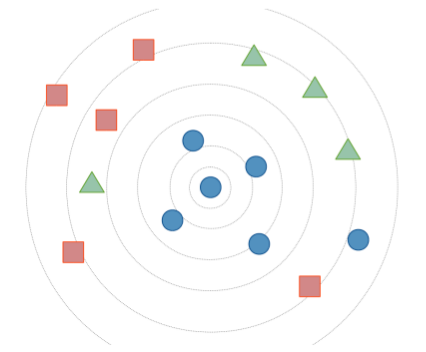
\includegraphics[scale=0.5]{pasta1_figuras/knn.png}
	\caption{Princípio dos k-vizinhos mais próximos}
	\label{fig-knn}
\end{figure}

Para encontrar os vizinhos mais próximos é necessário definir uma medida de similaridade entre dois exemplos. Uma medida de similaridade bastante popular é a \textit{distância euclidiana}. Tal medida calcula a raiz quadrada da norma do vetor diferença entre os vetores $x$ e $y$:
\begin{equation} \label{eq_disteucli}
d(x,y)= \sum_{i=1}^{K} (x_i - y_i)^2
\end{equation}

\section{Redes Neurais Artificiais}
Redes Neurais Artificais são modelos computacionais que buscam simular o processamento de informação pelo cérebro humano. Elas são compostas por unidades simples de processamento, os neurônios, que se unem por meio de conexões sinápticas \cite{zhang1998}. Cada conexão, além de ser altamente especializada, é responsável pelo envio de sinais de um neurônio para outro. Segundo \cite{haykin2009}, os neurônios e suas conexões podem ser implementados utilizando-se de componentes eletrônicos ou via simulação programada em computador.

\subsection{Inspiração Biológica e Perceptron}

Um bloco básico de uma rede neural tem algumas semelhanças com um neurônio biológico. O neurônio biológico é uma célula formada por três seçoes com funções específicas e complementares: \textit{corpo},\textit{dentritos} e \textit{axônio}. Os dentritos captam os estímulos recebidos em um determinado período de tempo e os transmitem ao corpo do neurônio, onde são processados. Quando tais estímulos atingirem determinado limite, o corpo da célula envia um novo impulso que se propaga pelo axônio e é transmitido às células vizinhas por meio de sinapses.  Este processo pode se repetir em várias camadas de neurônios. Como resultado, a informação de entrada é processada, podendo levar o cérebro a comandar reações físicas.  \cite{ferneda2006}. A figura \ref{fig-neuronio} ilustra de forma simplificada as partes de um neurônio.

\begin{figure}[h]
	\centering
	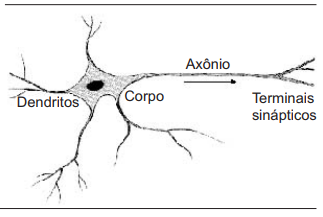
\includegraphics[scale=0.5]{pasta1_figuras/neuronio.png}
	\caption{Representação simplificada de um neurônio}
	\label{fig-neuronio}
\end{figure}

O modelo de um neurônio artifical é apresentado na Figura \ref{fig-guide-1}. Este modelo é composto por três elementos:
\begin{itemize}
	\item Um cojunto de entradas $(x_1,x_2,...,x_n)$ que são multiplicadas por um conjunto e pesos $(p_1,p_2,...,p_n)$;
	\item Um somador $(\sum)$ para acumular o sinais de entrada;
	\item Uma função de ativação que ($\varphi$) limita o intervalo permissível de amplitude do sinal de saída (y) a um valor fixo.
\end{itemize}

\textbf{\begin{figure}[h]
	\centering
	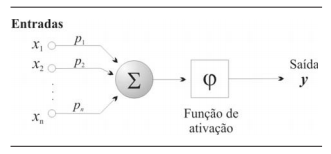
\includegraphics[scale=0.6]{pasta1_figuras/perceptron.png}
	\caption{Modelo matemátiico de um neurônio}
	\label{fig-perceptron}
\end{figure}}

Esse modelo foi proposto por \textit{McCulloch and Pitts} em 1943 \cite{McCulloch1943} e é conhecido como \textit{perceptron}. A função de ativação ($\varphi$) tem a seguinte definição:
\begin{equation} \label{eq_activation}
\varphi = \left\{ \,
\begin{IEEEeqnarraybox}[][c]{l?s}
\IEEEstrut
1 & if $\sum_{i=1}^{n} p_i x^k_i \geq T$, \\
0 & if $\sum_{i=1}^{n} p_i x^k_i < T$ 
\IEEEstrut
\end{IEEEeqnarraybox}
\right.
\end{equation}
Os valores dos pesos podem ser positivos ou negativos e eles refletem se aquela conexão é inibitória ou excitatória. Um valor positivo ou negativo reflete a importância da respectiva entrada para o processamento. Frequentemente é adicionado um \textit{viés} $b$ na entrada da função de ativação. A forma geral do modelo é descrito como:
\begin{equation} \label{eq-output-percep}
y(k) = \varphi(\sum_{i=1}^{n} p_i(k) x_i(k) +b(k))
\end{equation}
Os pesos sinápticos do Perceptron podem ser adaptados empregando um processo de aprendizado com um número finito de iterações. A aprendizagem é conduzida pela regra de correção de erro conhecida como algoritmo de convergência do Perceptron. Esse algoritmo visa encontrar um vetor de pesos w tal que as duas igualdades da função degrau sejam satisfeitas(\textit{Lippmann}, 1987 \cite{lippman1987})

\subsection{Perceptron multicamadas}

O Perceptron multicamadas(\textit{Multi-Layer Perceptron - MLP}) é uma generalização da rede perceptron. Novas camadas são adicionadas o que possibilita a solução de problemas que não sejam linearmente separáveis. O vetor de entradas \textbf{x} passa pela camada inicial, cujos valores de saída são ligados a camada seguinte. Esse processo se repete até chegar na última camada.(Figura \ref{fig-mlp})  Pode-se arranjar a rede em várias camadas, tornando-a profunda e capaz de aprender relações cada vez mais complexas.

\begin{figure}[h]
	\centering
	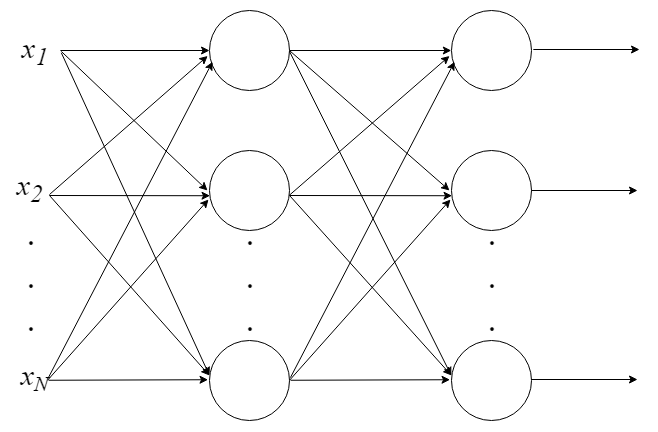
\includegraphics[scale=0.4]{pasta1_figuras/mlp.png}
	\caption{Multilayer Perceptron. Cada círculo representa um neurônio mostrado anteriormente}
	\label{fig-mlp}
\end{figure}

Em 1986, \textit{Rumelhart, Hinton e Williams} \cite{hinton1986} desenvolveram o algoritmo \textit{backpropagation}, que permite treinar uma MLP. Este método é composto pelas fases \textit{forward} e \textit{backward}.O objetivo do backpropagation é otimizar os pesos para que a rede neural possa aprender a mapear corretamente as entradas para as saídas. A primeira fase é a ``propragação adiante'' (forward), onde as entradas inseridas na rede se propagam entre as camadas, uma a uma, até a produção das respectivas saídas, portanto a função dessa fase é gerar uma resposta considerando as entradas e os respectivos pesos sinápticos, os quais permanecem inalterados.

Em seguida, essa resposta é então comparada com a saída desejada e um sinal de erro é calculado para cada elemento de saída. O sinal de erro é então retro-propagado da camada de saída para cada elemento da camada intermediária anterior que contribui diretamente para a formação da saída. Cada elemento da camada intermediária recebe apenas uma porção do sinal de erro total, proporcional apenas à contribuição relativa de cada elemento na formação da saída original. Este processo se repete, camada por camada, até que cada elemento da rede receba um sinal de erro que descreva sua contribuição relativa para o erro total. Baseado no sinal de erro recebido, os pesos das conexões são então atualizados para cada elemento de modo a fazer a rede convergir para um estado que permita a codificação de todos os padrões do conjunto de treinamento.

\section{Séries Temporais}

Série temporal é uma sequência de observações de um fenômeno ao longo do tempo. Geralmente essas medições são feitas em um intervalo de tempo regular. A ordem das amostras é crucial, pois há um dependência entre os dados e uma alteração da ordem pode modificar o significado dos dados. Uma série temporal pode ser definida como:

\begin{equation} \label{eq_TS}
X(t) = (x_1,x_2,...,x_n)
\end{equation}
onde $x_n$ representa uma observação no instante $t$, $n$ o número de observações e $X(t)$ a função que descreve a série temporal em termos de t. Caso a série seja constituída de uma observação em cada instante de tempo ela é chamada de \textit{univariada}. Caso a série foi obtida por uma coleta simultânea de dois ou mais fenômenos ela é chamada de \textit{multivariada}.

As séries temporais estão em diversas áreas do conhecimento como Economia (preços diários dea ações, taxa mensal de desemprego, produção industrial), Medicina (eletrocardiograma, eletroencefalograma), Epidemiologia (número mensal de novos casos de meningite), Meteorologia( precipitação pluviométrica, temperatura diária, velocidade do vento).

\subsection{Aplicações de Séries Temporais}
A análise de séries temporais tem atraído muitos pesquisadores em aprendizado de máquina ao redor do mundo. As principais tarefas envolvendo séries temporais na qual se utiliza aprendizagem de máquina são as seguintes:

\begin{itemize}
	\item \textit{Classificação}: cada série temporal representa uma classe distinta de objetos. Dada uma série temporal, o objetivo é descobrir qual é a classe de objetos ela representa; 
	\item Agrupamento: Dado um conjunto de séries temporais, o objetivo é encontrar uma estrutura natural que permita distribuir as séries em grupos; 
	\item Detecção de Motivos: também conhecido como detecção de \textit{motifs}; o objetivo é encontrar uma ou mais subsequências que aparecem frequentemente na séries;
	\item Detecção de Anomalias: encontrar subsequências ou séries que são inesperadas em algum contexto.
\end{itemize}
Este trabalho está inserido na tarefa de classificações de séries temporais.
\section{Classificação de Séries Temporais}


\section{Frequência Fundamental}

A frequência fundamental $f_0$ é a menor frequência de uma vibração, ou também, a primeira frequência de uma série harmônica. Uma série harmônica é o conjunto de ondas composto pela $f_0$ e suas múltiplas inteiras. Normalmente, todo estímulo sonoro é formado por uma série harmônica. A frequência fundamental está diretamente ligada à altura de um som e, por meio dela, distingue-se grave e agudo.


\section{Pitch}


O $pitch$ é um conceito musical relacionado à frequência fundamental, entretanto voltado para a percepção humana do som. Ele é definido em \cite{hartmann1996} como \textit{``o atributo pelo qual a audição pode ordenar os sons em uma escala de grave para agudo, dependendo principalmente do conteúdo de frequência do estímulo sonoro, mas também da forma de onda desse estímulo''}. Embora pareça confusa, esta definição abrange a relação do $pitch$ com a altura e com o timbre de um som, necessário para que o conceito seja válido em todos os casos, tanto em aplicações musicais como em aplicações de reconhecimento de fala. Em \cite{klapuri2006}, fica evidente que o $pitch$ de um som refere-se a frequência em que uma onda senoidal é reconhecida por um ouvido humano como correspondente ao som em questão.


\section{Detecção Automática de $f_0$}

Embora muitos trabalhos tratem frequência fundamental e $pitch$ como sinônimos, \cite{gerhard2003} explica de modo claro que existem diferenças consideráveis entre os dois conceitos, de modo que um sistema de detecção de $pitch$ objetiva resultados diferentes de um sistema de detecção de $f_0$. Como exemplo disso, pode-se observar que um sinal com frequências mais puras e poucas informações de timbre são ideais para a detecção de $f_0$, entretanto, a detecção de $pitch$ depende ainda da intensidade, duração e timbre.


Muitas soluções e métodos de detecção automática de $f_0$ já foram desenvolvidas e apresentadas, obtendo resultados positivos. Entretanto, \cite{gerhard2003} também afirma que é difícil que uma mesma solução de detecção de $f_0$ tenha bom desempenho tanto aplicações de música quanto em aplicações de fala. Deste modo, primeiro torna-se necessário definir o tipo de aplicação do sistema de detecção para, só então, desenvolver e avaliar o desempenho desse sistema no contexto escolhido.


\section{Digitalização de um Sinal de Som}

Para a digitalização de um sinal sonoro, são necessários a amostragem, a quantização e a codificação. 

\subsection{Amostragem}
A amostragem é o processo de conversão de um sinal contínuo no tempo em um sinal discreto. Se a discretização no tempo ocorrer em uma frequência de amostragem ($f_s$) muito baixa, as altas frequências não serão amostradas, gerando o efeito \textit{aliasing}, que é a distorção de um sinal causado pela perda das informações de alta frequência. 


Segundo o Teorema da Amostragem\cite{lathi2007}, dado um sinal contínuo amostrado com frequência $f_s$, se $f_s > 2f_M$, onde $f_M$ é a frequência máxima do sinal, então será possível recuperar toda a informação do sinal a partir dos valores amostrados. O intervalo entre a coleta de cada amostra é denominado \textit{período de amostragem}, representado pelo símbolo $T_s$. Pela relação de período e frequência, temos que $T_s = \frac{1}{f_s}$.


A Figura \ref{fig-sampling} demonstra graficamente a amostragem de um sinal.


\subsection{Quantização}
A quantização, por sua vez, consiste em selecionar um conjunto de valores finitos, espaçados linearmente ou não, para os quais as amostras terão seus valores de amplitude arredondados. A diferença entre o valor real e o valor quantizado da amostra é chamado de erro de quantização. Na digitalização de sinais, deve-se adotar um conjunto de quantização com tamanho suficientemente grande para que as perdas de informação por erros nesse procedimento não impeçam uma posterior recuperação do sinal.


A Figura \ref{fig-quantizacao} demonstra graficamente a quantização de um sinal.

\begin{figure}[h]
	\begin{subfigure}{0.5\textwidth}
		\centering
		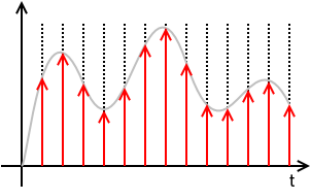
\includegraphics[scale=0.4]{pasta1_figuras/amostragem.png}
		\caption{Amostragem} \label{fig-sampling}
	\end{subfigure}
	\hspace*{\fill} % separation between the subfigures
	\begin{subfigure}{0.5\textwidth}
		\centering
		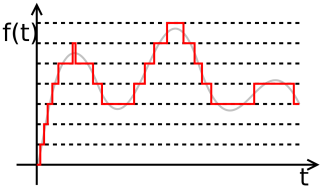
\includegraphics[scale=0.75]{pasta1_figuras/quantization.png}
		\caption{Quantização} \label{fig-quantizacao}
	\end{subfigure}
	\caption{Amostragem e Quantização}
\end{figure}

\subsection{Codificação}
Por fim, a codificação é o procedimento no qual se define o formato de armazenamento das informações do sinal. Após esse passo, essa representação digital passa a ser denominada áudio. Existem diferentes codificadores para áudio, cada um deles com suas particularidades. Alguns codificadores usam técnicas de compressão, que podem gerar pequenas perdas de informação, enquanto outros buscam preservar a integridade da representação, sendo, consequentemente, maiores em tamanho de arquivo. O Matlab\rreg trabalha nativamente com 8 tipos de codificadores de áudio: \textit{WAVE, OGG, FLAC, AU, AIFF, AIFC, MP3 e MPEG-4 AAC}\cite{mathworks2018audioread}.


\section{Notas Musicais}

Sob a ótica da música, os \textit{pitches} são representados pelas notas musicais. A distância entre a frequência de uma nota e metade ou dobro dessa mesma frequência é chamada de oitava. O menor intervalo entre duas notas é chamado de ``semitom'', enquanto um ``tom'' são dois semitons. A Tabela \ref{tab-notas} exibe todas as notas da 4ª oitava. A nota Lá (A) nessa oitava equivale a frequência de 440Hz, isso significa que essa mesma nota na 3ª oitava tem metade dessa frequência, ou seja, 220Hz. Por padrão, a nota lá da 4ª oitava, ou A4, é usada como base para a definição de todas as outras notas. A maioria dos músicos utiliza A4 em 440Hz, mas há casos em que são adotadas frequências diferentes como 436Hz e 444Hz.

\begin{table}[]
	\centering
	\begin{tabular}{|c|c|c|}
		\hline
		\textbf{Nota}                                           & \textbf{Abreviação} & \textbf{Frequência (em Hz)} \\ \hline
		Dó                                                      & C                   & 261.6                       \\ \hline
		\begin{tabular}[c]{@{}c@{}}Dó Sustenido ou Ré Bemol\end{tabular}  & C\# ou Db                 & 277.2                       \\ \hline
		Ré                                                      & D                   & 293.7                       \\ \hline
		\begin{tabular}[c]{@{}c@{}}Ré Sustenido ou Mi Bemol\end{tabular}  & D\# ou Eb                 & 311.1                       \\ \hline
		Mi                                                      & E                   & 329.6                       \\ \hline
		Fá                                                      & F                   & 349.2                       \\ \hline
		\begin{tabular}[c]{@{}c@{}}Fá Sustenido ou Sol Bemol\end{tabular}  & F\# ou Gb                 & 370.0                       \\ \hline
		Sol                                                     & G                   & 392.0                       \\ \hline
		\begin{tabular}[c]{@{}c@{}}Sol Sustenido ou Lá Bemol\end{tabular} & G\# ou Ab                 & 415.3                       \\ \hline
		Lá                                                      & A                   & 440.0                       \\ \hline
		Lá Sustenido ou Si Bemol                                            & A\# ou Bb                 & 466.2                       \\ \hline
		Si                                                      & B                   & 439.9                       \\ \hline
	\end{tabular}
	\caption{Notas musicais da 4ª oitava e suas frequências}
	\label{tab-notas}
\end{table}


\section{Ressonância}


A ressonância é um fenômeno físico em que uma vibração dá origem a outras vibrações com maior amplitude em um conjunto de frequências específicas. Essas frequências geradas são chamadas de frequências ressonantes. Os instrumentos musicais também podem apresentar esse fenômeno, como, por exemplo, alguns instrumentos de corda (violão, piano acústico, violino, entre outros) que utilizam uma caixa de ressonância para amplificar o som gerado pela vibração de suas cordas.


\section{Domínios}

Em PDS, os sinais são representados em dois diferentes domínios: tempo e frequência. No domínio do tempo, ou domínio temporal, um sinal é representado como amostragens de sua amplitude em intervalos de tempo $T$. Já no domínio da frequência, ou domínio espectral, um sinal é representado pela amplitude das oscilações que ocorrem em cada frequência. Desse modo, ter o mesmo sinal em diferentes domínios é tê-lo em diferentes perspectivas.


Os domínios do tempo e da frequência são permutáveis entre si, ou seja, dado um sinal $x(t)$ temporal, é possível transportar esse sinal para a representação espectral na forma $X(j\omega)$ sem que haja perda da informação. Do mesmo modo, é possível fazer o caminho inverso e retornar um sinal na frequência para a sua forma temporal inicial. Para transitar entre os domínios, utiliza-se as transformadas de Fourier.

\section{Transformada de Fourier}

A transformada de Fourier é uma ferramenta de decomposição de uma função em partes de base senoidal, ou seja, o sinal temporal passa a ser expresso em frequências. Inicialmente proposta pelo francês Jean Baptiste Joseph Fourier\cite{open1999}, as séries de Fourier deram origem a diferentes versões da transformada de Fourier, cada uma voltada para um tipo de sinal de origem.



Para sinais discretos no tempo utiliza-se a Transformada de Fourier em Tempo Discreto (DTFT, do inglês \textit{Discrete-Time Fourier Transform}), dada pela equação (\ref{eq_DTFT}):

\begin{equation} \label{eq_DTFT}
	X(\omega) = \sum_{n=-\infty}^{+\infty}x(n)e^{-j\omega n}
\end{equation}
onde $\omega$ é a frequência angular, em radianos por segundos, e $n$ é a posição da enésima amostra do sinal.


A DTFT é aplicável a sinais discretos no tempo, entretanto, é computacionalmente inviável, visto que sua saída é contínua na frequência. Deste modo, torna-se necessário discretizar essa saída para valores específicos de $\omega$. Para este fim, desenvolveu-se a Transformada Discreta de Fourier (DFT, do ingês \textit{Discrete Fourier Transform}).


\section{Transformada Discreta de Fourier}


A DFT é dada pela equação (\ref{eq_DFT}):

\begin{equation} \label{eq_DFT}
	X(k) = \sum_{n=0}^{N-1}x(n)e^{-j2\pi \frac{kn}{N}}
\end{equation}
onde x(n) é um sinal finito de tamanho N, e k assume valores inteiros de 0 a N-1.


Nesse contexto, X(k), DFT do sinal de entrada, é uma saída periódica. Essa discretização da saída aproxima a transformação de Fourier para a viabilidade computacional. Entretanto, executar uma soma do tamanho do sinal sob análise para cada valor específico da DFT,  ainda demanda um grande trabalho computacional, pois à medida em que aumenta-se o sinal de entrada, também aumenta-se quadraticamente a quantidade de operações. Por notação assintótica, pode-se afirmar que a DFT exige um esforço computacional $\Omega(N^2)$.


Por esse motivo, tornou-se necessário obter um algoritmo computacionamente mais eficiente para calcular a DFT: A Transformada Rápida de Fourier (FFT, do inglês \textit{Fast Fourier Transform}).


\section{Transformada Rápida de Fourier}

Designa-se como FFT uma série de algoritmos propostos que visam realizar a DFT de maneira mais eficiente. A Transformada Rápida de Fourier reduz as operações computacionais de $\Omega(N^2)$ para $\Omega( N log_2 N)$, tornando viável tal implementação. Para o presente projeto, utilizou-se a função nativa \textit{fft} do MATLAB\rreg, cujo a documentação fornece também casos básicos de uso\cite{mathworks2018}. Essa implementação baseia-se na equação:

\begin{equation} \label{eq-fft-matlab}
	X(k)=\sum_{j=1}^{N}x(j) W(N,j,k)
\end{equation}
onde $x(n)$ é o sinal de entrada, $N$ o tamanho do sinal, e $W$ é dado como:
\begin{equation} \label{eq-fft-matlab-w}
	W(N,j,k) = cos(\frac{2\pi i(j,k)}{N}) + j sen(\frac{2\pi i(j,k)}{N})
\end{equation}
onde,
\begin{equation} \label{eq-fft-matlab-i}
	i(j,k) = (j-1)(k-1)
\end{equation}

O tempo de execução dessa função depende do tamanho da entrada. Sinais com comprimentos que sejam potências de 2 são mais rápidos para o processamento, seguidos pelos sinais cujo o comprimento contém apenas pequenos fatores primos. As entradas que demoram mais para serem processadas são aquelas em que seu comprimento contém grandes fatores primos.


O tamanho e a precisão na frequência da saída de um algoritmo FFT também está diretamente relacionado ao tamanho do sinal de entrada. Em casos onde o sinal a ser transformado não possui um tamanho ideal para a precisão no domínio da frequência e tempo de execução desejados, pode-se adotar a técnica de \textit{padding}, acrescentando zeros ao final do sinal. 


\section{Transformada de Fourier de Tempo Curto}

A Transformada de Fourier de Tempo Curto (STFT, do inglês \textit{Short-time Fourier Transform}), é uma técnica de aplicação da transformada de Fourier utilizada para a análise de sinais não periódicos. Ela consiste na utilização de uma janela de tempo curto, que é colocada sobre o início do sinal. O segmento interno da janela é considerado como periódico e é submetido à transformada de Fourier. Após, desloca-se a janela de tempo curto e repete-se o processo até que a janela alcance o fim do sinal. Desse modo, é possível entender como o espectro de um sinal se comporta a cada instante de tempo. 


A STFT discreta pode ser implementada utilizando a FFT. O comprimento das janelas de tempo curto precisa ser definido conforme o tipo de aplicação desejada, pois deve ser compatível com o tamanho do fenômeno que deseja-se observar. Outro fator importante a ser definido é a forma de deslocamento da janela. Quando o tamanho da janela é igual ao valor de deslocamento, todas as amostras são analisadas uma única vez. Se o tamanho da janela for menor que o deslocamento, algumas amostras não serão analisadas, e se o deslocamento for maior, cada amostra será analisada em mais de uma posição da janela.


Em PDS, mais precisamente em sistemas de reconhecimento e detecção por áudio, essa técnica se torna imprescindível, pois permite uma visão clara da informação contida no sinal. 

\section{Espectrograma}

O espectrograma é uma forma de representar sinais. Ele mostra como o sinal evolui na frequência conforme o tempo. Existem diferentes formatos de gráfico para um espectrograma. A Figura \ref{fig-spectrogram} demonstra dois desses formatos: (a) e (b) Gráfico bidimensional com escala de cores, onde o eixo do tempo está na horizontal, o eixo da frequência na vertical e a amplitude é representada pela escala de cores; (c) e (d) Gráfico tridimensional clássico $z = f(x,y)$, onde o tempo está no eixo x, y é a frequência e z é a amplitude;

\begin{figure}[h]
	\begin{subfigure}{0.5\textwidth}
		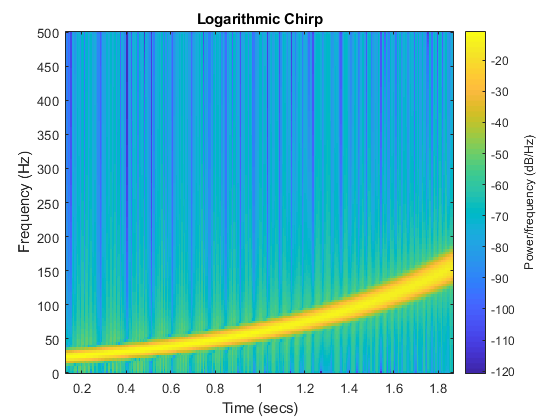
\includegraphics[scale=0.35]{pasta1_figuras/spectrogram1.png}
		\caption{}
	\end{subfigure}
	\hspace*{\fill} % separation between the subfigures
	\begin{subfigure}{0.5\textwidth}
		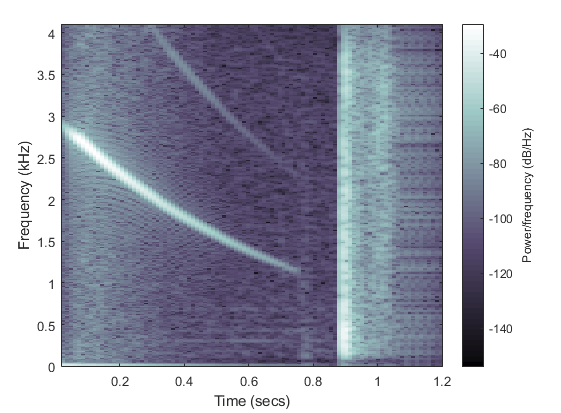
\includegraphics[scale=0.462]{pasta1_figuras/spectrogram4.png}
		\caption{}
	\end{subfigure}

	\begin{subfigure}{0.5\textwidth}
		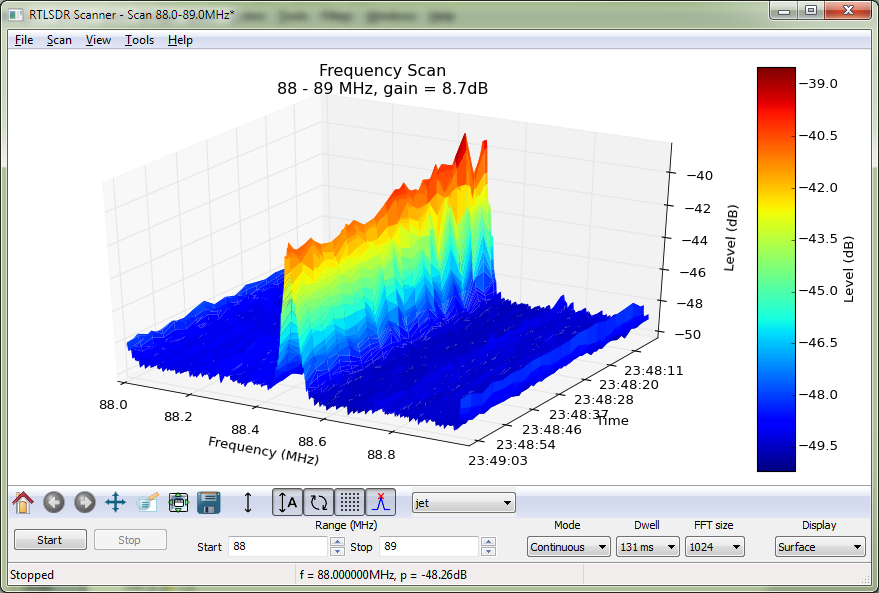
\includegraphics[scale=0.225]{pasta1_figuras/spectrogram2.png}
		\caption{}
	\end{subfigure}
	\hspace*{\fill} % separation between the subfigures
	\begin{subfigure}{0.5\textwidth}
	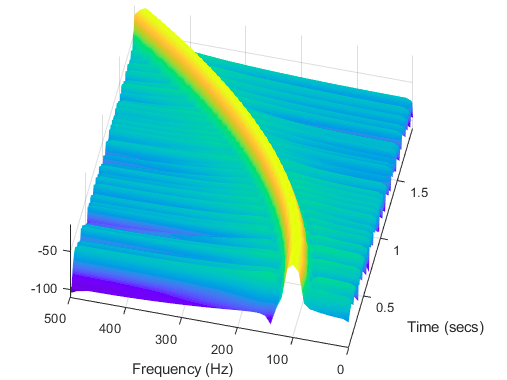
\includegraphics[scale=0.44]{pasta1_figuras/spectrogram3.png}
	\caption{}
	\end{subfigure}
	 \caption{Espectrogramas no MATLAB\rreg} \label{fig-spectrogram}
\end{figure}

O método mais usual para a geração do espectrograma de um sinal é por meio da STFT. Aplicando a técnica, calcula-se a FFT de cada janela do sinal de entrada. Como a saída da FFT pode conter números complexos, computa-se o módulo dos valores de saída da transformada, obtendo-se vários planos de frequências e amplitudes. Por fim, os planos de espectro de cada janela de tempo são colocados lado a lado, formando assim o espectrograma completo.


A equação (\ref{eq-spectrogram}) descreve esse processo com o uso da STFT:

\begin{equation}
	\label{eq-spectrogram}
	spectrogram(x(n), \Delta) = |STFT(x(n),\Delta)|^2
\end{equation}
onde $x(n)$ é o sinal sob análise e $\Delta$ é o tamanho da janela para a STFT.


O MATLAB\rreg fornece o método \textit{spectrogram} para obter, por meio da STFT, o espectrograma de um sinal\cite{mathworks2018spectrogram}. Este método utiliza por padrão o gráfico bidimensional com escala de cores.

%[Detecção de oitavas]
%[Problemas de continuidade]

%\section{Ruído}

%Indicar quais são os quais são os principais fundamentos (algoritmos, paradigmas, teorias) a serem empregados.
%Cada fundamento utilizado deve ser justificado.


% Fim Capítulo